% \pdfoutput=1    % apparently this is needed at the beginning for arXiv to process it

% \documentclass[letterpaper, 10 pt, conference]{ieeeconf}
\documentclass[letterpaper, 10 pt, journal, twoside]{IEEEtran}


\IEEEoverridecommandlockouts                              % This command is only needed if 
                                                          % you want to use the \thanks command

% \overrideIEEEmargins                                      % Needed to meet printer requirements. Comment this for final RAL version, but keep it for final conference version.

% numbers option provides compact numerical references in the text. 
% \usepackage[numbers]{natbib}
\usepackage{multicol}
\usepackage[bookmarks=true]{hyperref}

% Various packages
\usepackage{float}
\usepackage{comment}
\usepackage{array}
\usepackage{graphicx}
\usepackage{booktabs}
\usepackage{multirow}

% Various math packages
\usepackage{amsmath}								
\usepackage{amssymb}
\usepackage{latexsym}
\usepackage{amsthm}
\usepackage{bm}
\usepackage{commath}
\usepackage{float}
\usepackage{units}

% packages for drawings
\usepackage{tikz}
% \usetikzlibrary{external}
% \tikzexternalize[prefix=tikz/] % activate!
\usetikzlibrary{arrows,shapes,trees,calc}
\usetikzlibrary{backgrounds}
\usepackage{pgfplots}
\pgfplotsset{compat=1.14}
\usepgfplotslibrary{polar}
\usepgfplotslibrary{patchplots}

% % reduce white space after captions
% \setlength{\textfloatsep}{10pt}

%% downsample images to make file smaller
%\usepackage{epstopdf}
%\epstopdfDeclareGraphicsRule{.pdf}{png}{.png}{convert #1 \OutputFile}
%\DeclareGraphicsExtensions{.png,.pdf}

% packages for 3d plotting with tikz
\usepackage{tikz-3dplot} %requires 3dplot.sty to be in same directory, or in your LaTeX installation
%\usepackage[active,tightpage]{preview}  %generates a tightly fitting border around the work
%\PreviewEnvironment{tikzpicture}
%\setlength\PreviewBorder{2mm}

% Commands for theorems
\newtheorem{definition}{Definition}[section]
\newtheorem{theorem}{Theorem}[section]
\newtheorem{assumption}{Assumption}[section]

% Definitions of custom colors
\definecolor{lightyellow}{RGB}{255,236,132}
\definecolor{lightgreen}{RGB}{161,239,10}
\definecolor{darkgreen}{RGB}{61,124,68}
\definecolor{lightblue}{RGB}{72,131,219}
\definecolor{darkblue}{RGB}{39,63,186}
\definecolor{plgreen}{RGB}{27,158,119}
\definecolor{plorange}{RGB}{217,95,2}
\definecolor{plpurple}{RGB}{117,112,179}
\definecolor{plpink}{RGB}{231,41,138}


% Editing tools
\usepackage{color}  % For Highlighting
\newcommand{\hilight}[1]{\colorbox{yellow}{#1}}
\newcommand{\David}[1]{\textcolor{red}{(#1)}}
\newcommand{\Ram}[1]{\textcolor{blue}{(#1)}}
\newcommand{\Dan}[1]{\textcolor{magenta}{(#1)}}
\newcommand{\Audrey}[1]{\textcolor{maroon}{(#1)}}

% Set macros to make certain things easier
\newcommand{\bmx}{\begin{bmatrix}}
\newcommand{\emx}{\end{bmatrix}}
\newcommand{\D}{\bar{\mathcal{D}}}

% Load and define stuff needed to add labels in the margins
\usepackage{marginnote}
% \makeatletter
% \let\oldmarginnote\marginnote
% \renewcommand*{\marginnote}[1]{%
%   \begingroup%
%   \ifodd\value{page}
%      \if@firstcolumn\reversemarginpar\fi
%   \else
%      \if@firstcolumn\else\reversemarginpar\fi
%   \fi
%   \oldmarginnote{#1}%
%   \endgroup%
% }
% \makeatother

% Set macro for labeling edits
\newcommand{\revcomment}[2]{\textcolor{red}{#2} \marginnote{\##1}} % Include reference commands
\renewcommand{\revcomment}[2]{#2}   % removes coloring of edited sections, i.e. makes doc look normal (comment this line out for highlighted edits)


\title{\LARGE \bf
Force Generation by Parallel Combinations of \\ Fiber-Reinforced Fluid-Driven Actuators
}


\author{Daniel Bruder$^{1}$, %<-this % stops a space
        Audrey Sedal$^{1}$, %
        Ram Vasudevan$^{1}$, %
        and C. David Remy$^{1}$%
\thanks{Manuscript received: February, 25, 2018; Revised May, 29, 2018; Accepted July, 9, 2018.}    % use only for final RAL version
\thanks{This paper was recommended for publication by Editor Yu Sun upon evaluation of the Associate Editor and Reviewers' comments.
*This material is supported by the Toyota Research Institute, and is based upon work supported by the National Science Foundation Graduate Research Fellowship Program under Grant No. 1256260 DGE. Any opinions, findings, and conclusions or recommendations expressed in this material are those of the author(s) and do not necessarily reflect the views of the National Science Foundation.}% <-this % stops a space
\thanks{$^{1}$ The authors are with the Mechanical Engineering Department at the 
        University of Michigan, Ann Arbor, MI 48109, USA
        {\tt\small \{bruderd, asedal, ramv, cdremy\}@umich.edu}}%
\thanks{Digital Object Identifier (DOI): see top of this page.}
% \thanks{This work has been submitted to the IEEE for possible publication. Copyright may be transferred without notice, after which this version may no longer be accessible.}   % for archive version only
}

\begin{document}

\maketitle
% \thispagestyle{empty}         % commented for final RAL version
% \pagestyle{empty}             % commented for final RAL version

% Paper headers (for final RAL submission)
\markboth{IEEE Robotics and Automation Letters. Preprint Version. Accepted July, 2018}
{Bruder \MakeLowercase{\textit{et al.}}: Force Generation by Parallel Combinations of Fluid-Driven Actuators}  % Use only for final RAL version

\begin{abstract}
  In this paper, we explore the connection between secret key agreement and secure omniscience within the setting of the multiterminal source model with a wiretapper who has side information. While the secret key agreement problem considers the generation of a maximum-rate secret key through public discussion, the secure omniscience problem is concerned with communication protocols for omniscience that minimize the rate of information leakage to the wiretapper. The starting point of our work is a lower bound on the minimum leakage rate for omniscience, $\rl$, in terms of the wiretap secret key capacity, $\wskc$. Our interest is in identifying broad classes of sources for which this lower bound is met with equality, in which case we say that there is a duality between secure omniscience and secret key agreement. We show that this duality holds in the case of certain finite linear source (FLS) models, such as two-terminal FLS models and pairwise independent network models on trees with a linear wiretapper. Duality also holds for any FLS model in which $\wskc$ is achieved by a perfect linear secret key agreement scheme. We conjecture that the duality in fact holds unconditionally for any FLS model. On the negative side, we give an example of a (non-FLS) source model for which duality does not hold if we limit ourselves to communication-for-omniscience protocols with at most two (interactive) communications.  We also address the secure function computation problem and explore the connection between the minimum leakage rate for computing a function and the wiretap secret key capacity.
  
%   Finally, we demonstrate the usefulness of our lower bound on $\rl$ by using it to derive equivalent conditions for the positivity of $\wskc$ in the multiterminal model. This extends a recent result of Gohari, G\"{u}nl\"{u} and Kramer (2020) obtained for the two-user setting.
  
   
%   In this paper, we study the problem of secret key generation through an omniscience achieving communication that minimizes the 
%   leakage rate to a wiretapper who has side information in the setting of multiterminal source model.  We explore this problem by deriving a lower bound on the wiretap secret key capacity $\wskc$ in terms of the minimum leakage rate for omniscience, $\rl$. 
%   %The former quantity is defined to be the maximum secret key rate achievable, and the latter one is defined as the minimum possible leakage rate about the source through an omniscience scheme to a wiretapper. 
%   The main focus of our work is the characterization of the sources for which the lower bound holds with equality \textemdash it is referred to as a duality between secure omniscience and wiretap secret key agreement. For general source models, we show that duality need not hold if we limit to the communication protocols with at most two (interactive) communications. In the case when there is no restriction on the number of communications, whether the duality holds or not is still unknown. However, we resolve this question affirmatively for two-user finite linear sources (FLS) and pairwise independent networks (PIN) defined on trees, a subclass of FLS. Moreover, for these sources, we give a single-letter expression for $\wskc$. Furthermore, in the direction of proving the conjecture that duality holds for all FLS, we show that if $\wskc$ is achieved by a \emph{perfect} secret key agreement scheme for FLS then the duality must hold. All these results mount up the evidence in favor of the conjecture on FLS. Moreover, we demonstrate the usefulness of our lower bound on $\wskc$ in terms of $\rl$ by deriving some equivalent conditions on the positivity of secret key capacity for multiterminal source model. Our result indeed extends the work of Gohari, G\"{u}nl\"{u} and Kramer in two-user case.
\end{abstract}

% Keywords appear just beneath the abstract. Use only for final RAL version.
\begin{IEEEkeywords}
Soft Material Robotics, Hydraulic/Pneumatic Actuators, Force Control
\end{IEEEkeywords}

\IEEEpeerreviewmaketitle

% % !TEX root = main.tex

\section{Proof of Proposition~\ref{propEssTightness}}

%RECALL PROBLEM
%BIG IDEA: LEVEL-CROSSING UNDER UNCONDITIONAL MEASURE
The challenge of Proposition~\ref{propEssTightness} is to establish bounds on the defects $\sigma(x) - \t(x)$ for sites $x$ far away from the origin.
The essence of the proof of Proposition~\ref{propEssTightness} is a carefully devised level-crossing argument leveraging the renewal structure of standard hitting times under the unconditioned measure $\P$. To achieve this goal, we introduce variants of the times $\{u_n, v_n\}_{n\ge1}$ from Section~\ref{essHitSec} that are tailor-made for the purpose of our proof.

%TAKE LARGE BALL AROUND x
%IF AT LEAST ONE SHELL GENERATES SURVIVING INFECTION => USE GM
More precisely, after fixing $L$ as in the statement of the proposition, we consider the ball 
$$B(x, R^2) = \{y \in \Zd:\, |y - x| \le R^2 \}$$
of radius $R^2$ around $x$, where $R$ is large and depends on $L$, but not on $x$. We pay special attention to the times at which the  infection hits each of the  $R$ shells 
$$\partial B(x,iR) = \{y \in \Zd: |y-x| = iR \},\quad 1\le i \le R. $$
If for some $i$ the space-time point where the infection hits the $i$th shell for the first time gives rise to a surviving contact process, then, by a renewal argument, it suffices to bound the essential hitting time of a point at distance at most $R^2$ from the origin. In particular, for this it is sufficient to invoke earlier location-dependent upper bounds.

%RENEWAL => PROBABILITY THAT ALL INFECTIONS DIE OUT DECAYS EXPONENTIALLY
The alternative is that upon hitting each of the $R$ shells, the infection started from the hitting point dies out. In the super-critical regime, a further renewal argument shows that this is an event of probability decaying geometrically in the number of shells. 


%RENEWAL REQUIRES RAPID DEATH OF NON-SURVIVING INFECTIONS
We clearly need a due amount of care in order to make the renewal argument rigorous. In particular, it is important to know that the infections starting from the hitting points die out before the next shell is reached.

Due to the regenerative arguments sketched above, we need the location-dependent bounds from~\cite[Theorem 15]{GaretMarch14} not only if the infection is started from the origin, but from an arbitrary set $A \subseteq \Zd$ with $o \in A$. More precisely, we now put $u^A_0(x) = v^A_0(x) = 0$ and
\[u^A_{k+1}(x)=\inf\{t\ge v^A_k(x):x\in\xi^A_t\},\]
whereas the recursion for $v^A_{k+1}$ is unchanged, i.e., 
\[v^A_{k+1}(x)=\sup\{s\ge0:\; (x,u^A_{k+1}(x)) \rightsquigarrow \Zd \times \{s\} \}. \]
Finally, we set $\sigma^A(x)=u_{K^A(x)}(x) $ where 
\[K^A(x)=\min\{n\ge0:v^A_n(x)=\infty\text{ or }u^A_n(x)=\infty\}.\]


%The proof is based on the shape theorem and the notion of essential hitting times.

\begin{lemma}
	\label{cor20}
There exist $c$, $c' > 0$ such that for all $L > 0$, $x \in \Zd$ and $A \subseteq \Zd$ with $o \in A$,
\begin{align}\label{eqcor20}
\oP\left(\sigma^A(x) > L\right) \leq \exp\{-cL + c'|x|\}.
\end{align}
\end{lemma}
%For $A = \{0\}$, this follows immediately from \cite[Corollary 20]{GaretMarch14}, the novelty being uniformity in the initial condition $A$. 
%In view of \cite[Corollary 20]{GaretMarch14}, it is plausible that $C$ may be chosen as a linear function of $\|x\|$; however, we do not need this to prove the (much stronger) bound of Proposition \ref{propEssTightness}. 
\begin{proof}
The result follows from Chebyshev's inequality and the claim that there exist $\beta, \gamma > 0$ such that, for all $x \in \Zd$ and all $A \subseteq \Zd$ with $o \in A$,
$$\oE(\exp\{\beta \sigma^A(x)\}) \leq \exp\{\gamma |x|\}. $$
	For the case $A = \{o\}$, this is \cite[Theorem 15]{GaretMarch14}. The statement with general $A \subseteq \Zd$ with $o \in A$ is proved in exactly the same way, so we do not go over the details.
\end{proof}


\begin{proof}[Proof of Proposition~\ref{propEssTightness}]
  Fix $L > 0$, which we may assume to be large throughout the proof without loss of generality. Define $R = \lfloor L^{1/4}\rfloor$. Let us first fix $x \in \Zd$ with $|x| \leq R^2$. Then, by Lemma~\ref{cor20},
\begin{equation}\oP(\sigma(x) - t(x) > L) \leq \oP(\sigma(x) > L) \stackrel{\eqref{eqcor20}}{\leq} \exp\left\{-cL + c'|x|\right\} < \exp\left\{-cL/2\right\}.\label{eq:zeroth_ing}\end{equation}

Now we fix $x$ with $|x| > R^2$ and aim to show that
\begin{equation}\label{eqDestBd}\P(\sigma(x) < \infty,\;\sigma(x) - t(x) > L) < C_0\exp\{-L^{\gamma_0}\}\end{equation}
for some $C_0,\gamma_0 > 0$; the desired bound then follows since $\oP(\sigma(x) < \infty) = 1$. As suggested in the outline of proof, we define the shell radius $r_i = R(R-i+1)$ and let
$$U_i = \inf\{t: \xi_t^o \cap B(x,r_i) \neq \varnothing\},\qquad i = 1,\ldots, R.$$
denote the first time that the infection hits the $i$th shell. On the event $\{U_i < \infty\}$, let $Z_i \in \partial B(x,r_i)$ denote the unique point of $\xi^o_{U_i} \cap B(x, r_i)$. Also on $\{U_i < \infty\}$, let
$$V_i = \inf\{s \geq U_i:\;(Z_i,U_i) \not\rightsquigarrow \Zd \times \{s\}\}$$
	denote the time at which  the infection starting from $(Z_i, U_i)$ dies out.

	Then there are three alternative scenarios under which the event $\{\sigma(x) < \infty,\;\sigma(x) - t(x) > L\}$ can occur: 
	\begin{enumerate}
		\item there exists at least one shell $\partial B(x, r_i)$ such that the infection generated by the first hitting point survives forever, i.e., $V_i = \infty$,
		\item for each $i \in \{1,\ldots, n\}$ the infection generated by the hitting point $(Z_i, U_i)$ dies out before the global infection reaches the $(i+1)$th shell, 
		\item one of these non-surviving infections lives longer than it takes the global infection to reach the next shell.
	\end{enumerate}
	More precisely,
\begin{equation}\label{eq:3terms}\begin{split}
\P(\sigma(x) < \infty,\; \sigma(x) - t(x) > L) &\leq \sum_{n=1}^R\P(U_n < \infty,\; V_n = \infty,\; \sigma(x) - t(x) > L) \\&+
 \P(U_1 < V_1 < U_2 < V_2 <\cdots < U_R < V_R < \infty)\\&
	+ \sum_{n=1}^{R-1} \P(U_{n+1} < V_{n} <\infty)
\end{split}\end{equation}
	We separately bound the three terms on the right-hand side. By repeated use of the Markov property, we have 
	\begin{equation}\P(U_1 < V_1 < U_2 < V_2 <\cdots < U_R < V_R < \infty)\leq(1-\rho)^R, \label{eq:first_ing}\end{equation} 
		where we recall that $\rho = \P_\lambda(o \rightsquigarrow \infty)$  denotes the survival probability. Next, for any $n$,
\begin{align}
&\P(U_n < \infty,\; V_n = \infty,\;\sigma(x) - t(x) > L) \leq \P(U_n < \infty,\;V_n = \infty,\;\sigma(x) - U_n > L) \nonumber\\
&=\sum_{y \in \partial B(x,r_n)}\; \sum_{\substack{A \subseteq \Zd,\\A\text{ finite}}} \P(U_n < \infty,\; Z_n = y,\; (y, U_n) \rightsquigarrow \infty,\; \xi^o_{U_n} = A,\; \sigma(x) - U_n > L)\nonumber\\
&= \sum_{y \in \partial B(x,r_n)}\; \sum_{\substack{A \subseteq \Zd,\\A \text{ finite}}} \P(U_n < \infty,\; Z_n = y,\;  \xi^o_{U_n} = A) \cdot \rho\cdot \oP(\sigma^{A-y}(x-y) > L)\nonumber\\
&\leq \rho \cdot \P(U_n < \infty) \cdot \exp\{-cL/2\},\label{eq:second_ing}
\end{align}
	the last inequality is obtained as in \eqref{eq:zeroth_ing} using $|x - y| \le R^2$. We now turn to the term inside the third sum on the right-hand side of \eqref{eq:3terms}. Since the contact process is in the super-critical regime, the survival time of a non-surviving infection started at a single site has exponential tails, cf.~\cite[Proposition 5]{GaretMarch12}, so that the Markov property yields
\begin{equation}\begin{split}\P(U_{n+1} < V_n < \infty) &\leq \P(V_n - U_n \in (\sqrt{R}, \infty)) + \P(U_{n+1} - U_n < 2\sqrt{R})\\
&\leq \exp\{-c\sqrt{R} \} + \P(\partial B(x,r_i) \times [0,2\sqrt{R}] \rightsquigarrow B(x,r_{i+1}) \times[0,2\sqrt{R}]).\end{split}\label{eq:third_ing}
\end{equation}
Since the propagation speed of the infection is at most linear outside an event of exponentially decaying probability ~\cite[Proposition 5]{GaretMarch12}, the second term on the right-hand side is less than
\begin{align}\nonumber&\#\partial B(x,r_i) \cdot 2d\lambda \cdot \int_0^{2\sqrt{R}} \max_{y \in \partial B(x,r_i)} \P\Big((y,s) \rightsquigarrow B(x,r_{i+1})\times [s,2\sqrt{R}] \Big)\; \mathrm{d}s
\\\nonumber&\leq \#\partial B(x,r_i) \cdot 2d\lambda \cdot 2\sqrt{R} \cdot \P\Big(\bigcup_{s \leq 2\sqrt{R}}\xi^y_s \nsubseteq B(y, R/2)\Big) \\&\leq \#\partial B(x,r_i) \cdot 2d\lambda \cdot 2\sqrt{R} \cdot \exp\{-c\sqrt{R}\}.\label{eq:third_ing0}
\end{align}
Combining the bounds \eqref{eq:3terms}, \eqref{eq:first_ing}, \eqref{eq:second_ing}, \eqref{eq:third_ing} and \eqref{eq:third_ing0} implies  \eqref{eqDestBd} and finishes the proof.
\end{proof}


% Input sections here
% \leavevmode
% \\
% \\
% \\
% \\
% \\
\section{Introduction}
\label{introduction}

AutoML is the process by which machine learning models are built automatically for a new dataset. Given a dataset, AutoML systems perform a search over valid data transformations and learners, along with hyper-parameter optimization for each learner~\cite{VolcanoML}. Choosing the transformations and learners over which to search is our focus.
A significant number of systems mine from prior runs of pipelines over a set of datasets to choose transformers and learners that are effective with different types of datasets (e.g. \cite{NEURIPS2018_b59a51a3}, \cite{10.14778/3415478.3415542}, \cite{autosklearn}). Thus, they build a database by actually running different pipelines with a diverse set of datasets to estimate the accuracy of potential pipelines. Hence, they can be used to effectively reduce the search space. A new dataset, based on a set of features (meta-features) is then matched to this database to find the most plausible candidates for both learner selection and hyper-parameter tuning. This process of choosing starting points in the search space is called meta-learning for the cold start problem.  

Other meta-learning approaches include mining existing data science code and their associated datasets to learn from human expertise. The AL~\cite{al} system mined existing Kaggle notebooks using dynamic analysis, i.e., actually running the scripts, and showed that such a system has promise.  However, this meta-learning approach does not scale because it is onerous to execute a large number of pipeline scripts on datasets, preprocessing datasets is never trivial, and older scripts cease to run at all as software evolves. It is not surprising that AL therefore performed dynamic analysis on just nine datasets.

Our system, {\sysname}, provides a scalable meta-learning approach to leverage human expertise, using static analysis to mine pipelines from large repositories of scripts. Static analysis has the advantage of scaling to thousands or millions of scripts \cite{graph4code} easily, but lacks the performance data gathered by dynamic analysis. The {\sysname} meta-learning approach guides the learning process by a scalable dataset similarity search, based on dataset embeddings, to find the most similar datasets and the semantics of ML pipelines applied on them.  Many existing systems, such as Auto-Sklearn \cite{autosklearn} and AL \cite{al}, compute a set of meta-features for each dataset. We developed a deep neural network model to generate embeddings at the granularity of a dataset, e.g., a table or CSV file, to capture similarity at the level of an entire dataset rather than relying on a set of meta-features.
 
Because we use static analysis to capture the semantics of the meta-learning process, we have no mechanism to choose the \textbf{best} pipeline from many seen pipelines, unlike the dynamic execution case where one can rely on runtime to choose the best performing pipeline.  Observing that pipelines are basically workflow graphs, we use graph generator neural models to succinctly capture the statically-observed pipelines for a single dataset. In {\sysname}, we formulate learner selection as a graph generation problem to predict optimized pipelines based on pipelines seen in actual notebooks.

%. This formulation enables {\sysname} for effective pruning of the AutoML search space to predict optimized pipelines based on pipelines seen in actual notebooks.}
%We note that increasingly, state-of-the-art performance in AutoML systems is being generated by more complex pipelines such as Directed Acyclic Graphs (DAGs) \cite{piper} rather than the linear pipelines used in earlier systems.  
 
{\sysname} does learner and transformation selection, and hence is a component of an AutoML systems. To evaluate this component, we integrated it into two existing AutoML systems, FLAML \cite{flaml} and Auto-Sklearn \cite{autosklearn}.  
% We evaluate each system with and without {\sysname}.  
We chose FLAML because it does not yet have any meta-learning component for the cold start problem and instead allows user selection of learners and transformers. The authors of FLAML explicitly pointed to the fact that FLAML might benefit from a meta-learning component and pointed to it as a possibility for future work. For FLAML, if mining historical pipelines provides an advantage, we should improve its performance. We also picked Auto-Sklearn as it does have a learner selection component based on meta-features, as described earlier~\cite{autosklearn2}. For Auto-Sklearn, we should at least match performance if our static mining of pipelines can match their extensive database. For context, we also compared {\sysname} with the recent VolcanoML~\cite{VolcanoML}, which provides an efficient decomposition and execution strategy for the AutoML search space. In contrast, {\sysname} prunes the search space using our meta-learning model to perform hyperparameter optimization only for the most promising candidates. 

The contributions of this paper are the following:
\begin{itemize}
    \item Section ~\ref{sec:mining} defines a scalable meta-learning approach based on representation learning of mined ML pipeline semantics and datasets for over 100 datasets and ~11K Python scripts.  
    \newline
    \item Sections~\ref{sec:kgpipGen} formulates AutoML pipeline generation as a graph generation problem. {\sysname} predicts efficiently an optimized ML pipeline for an unseen dataset based on our meta-learning model.  To the best of our knowledge, {\sysname} is the first approach to formulate  AutoML pipeline generation in such a way.
    \newline
    \item Section~\ref{sec:eval} presents a comprehensive evaluation using a large collection of 121 datasets from major AutoML benchmarks and Kaggle. Our experimental results show that {\sysname} outperforms all existing AutoML systems and achieves state-of-the-art results on the majority of these datasets. {\sysname} significantly improves the performance of both FLAML and Auto-Sklearn in classification and regression tasks. We also outperformed AL in 75 out of 77 datasets and VolcanoML in 75  out of 121 datasets, including 44 datasets used only by VolcanoML~\cite{VolcanoML}.  On average, {\sysname} achieves scores that are statistically better than the means of all other systems. 
\end{itemize}


%This approach does not need to apply cleaning or transformation methods to handle different variances among datasets. Moreover, we do not need to deal with complex analysis, such as dynamic code analysis. Thus, our approach proved to be scalable, as discussed in Sections~\ref{sec:mining}.
\section{Modeling}
\label{sec:singleActuator}
%
Our modeling approach for individual FREEs is based on the notion of a \emph{fluid Jacobian} $\bar{J}$, which maps the geometrical deformation of a soft actuator, or of a system of actuators, to a change in their volume. 
Under certain assumptions, the transpose of this Jacobian linearly maps the internal fluid pressure to the spatial forces that the actuator generates. 
One can  think of this fluid Jacobian as the soft and multi-dimensional equivalent of the cross section $A$ of a traditional pneumatic or hydraulic cylinder,
since this cross section similarly relates cylinder pressure to force, and piston movement to fluid displacement.


\subsection{Force Generation in a Single FREE}
%
The approach presented in this paper is enabled by a number of simplifying assumptions.
They are consistent with those made in prior work on the modeling and control of individual FREEs \cite{bishop2015design,bruder2017model}.
In particular, we assume that the fibers are inextensible and that they are uniformly  distributed  around  an elastomeric cavity  with negligible  wall thickness.
%The internal pressure in this cavity is uniform along its entire length.
Under these assumptions, a FREE can be modeled as a composition of an energy transforming element (the fibers) and an energy storing element (the compliance of the elastomer body). 
The generalized forces generated by each of these separate elements can be superimposed to characterize the net force $\vec{\tau}_{total}$ produced by the FREE:
\begin{align}
   \vec{\tau}_{\text{total}} &=  \vec{\tau} + \vec{\tau}_{\text{elast}}    \label{eq:netF}
\end{align}
where $\vec{\tau}$ and $\vec{\tau}_{\text{elast}}$ are the generalized forces and torques attributed to the fiber and elastomer, respectively.
In this work, we focus exclusively on the active general forces $\vec{\tau}$ that are generated by the fibers and that can be controlled by varying the pressure of the fluid.


The fluid Jacobian for such an actuator can be derived from the idea that the reinforcing fibers in a FREE create a kinematic constraint on the internal volume $V$ of the fluid cavity.
Without the reinforcing fibers, this cavity could expand freely, since it is made from soft material.
With the fibers, however, the volume is limited.
This limitation on volume depends on the mechanical parameters of the FREE (e.g., the relaxed fiber angle or fiber length) and on the current state of geometric deformation of the FREE.
This geometric state can be represented by a generalized vector of spatial deformations $\vec{q}$:  $V = V\left(\vec{q}\right)$.


The derivative of this volume yields an expression $\dot{V}$ for the volumetric flow into the actuator:
\begin{align}
    \dot{V} (\vec{q}, \dot{\vec{q}}) &= \frac{\partial V}{\partial t} = \frac{\partial V}{\partial \vec{q}} \frac{\partial \vec{q}}{\partial t } = \bar{J}_q (\vec{q}) \dot{\vec{q}},  \label{eq:Vdot_wJ}
\end{align}
where the fluid Jacobian is defined as $\bar{J}_{q}= \frac{\partial V}{\partial \vec{q}}$ with respect to the deformation $\vec{q}$. 


It is important to note that $\vec{\tau}$ and $\dot{\vec{q}}$ live in dual spaces. 
That is, forces in $\vec{\tau}$ correspond to linear motion in $\dot{\vec{q}}$, and moments in $\vec{\tau}$ correspond to angular motion in $\dot{\vec{q}}$.
In the most general case, these are 6-dimensional vectors with three translations and three rotations.
In this case, $\bar{J}_q$ is a $1 \times 6$ matrix.


Energy conservation dictates that the mechanical power generated by the fibers must equal the fluid power that goes into the FREE:
\begin{align}
    P_{\text{mech}} = P_{\text{fluid}} = \dot{\vec{q}}^{\,T} \vec{\tau} &= \dot{V} p, 
    \label{eq:Pequiv}
\end{align}
%
where $p>0$ is the pressure of the fluid inside the FREE.
Substituting \eqref{eq:Vdot_wJ} into \eqref{eq:Pequiv}, we arrive at a linear expression that yields the forces produced by the FREE fibers as a function of deformation state and fluid pressure: 
\begin{align}
    \vec{\tau} (\vec{q}, p) &= \bar{J}_q^T (\vec{q}) p       \label{eq:fiberF}
\end{align}
The fluid Jacobian thus describes the generalized direction in which a FREE can produce forces and torques.
Since the input pressure $p$ needs to be strictly positive to avoid collapsing of the fluid cavity, forces can only be produced in the positive direction defined by $\bar{J}_q$.


\subsection{The Fluid Jacobian of a Cylindrical FREE}
The theoretical modeling approach outlined above can be applied independently of the exact geometry of a FREE and can even be extended to other classes of soft actuators.
However, to make the computation of the fluid Jacobian tractable, we rely on another common assumption for FREES: that they maintain the geometry of an ideal cylinder \cite{bishop2015design}.
This neglects the tapering of the actuator towards the end-caps and any potential bending along its main axis.

\begin{figure}
    \centering
    \begin{tikzpicture}
        \node (FREEstate) at (0,0)
            {\includegraphics[width=0.75\linewidth]{figures/FREEstate_noLabels3.pdf}};
        \node[right] (a) at ($ (FREEstate.east) !0.5! (FREEstate.north east) $) {(a)};
        \node[right] (b) at ($ (FREEstate.east) !0.5! (FREEstate.south east) $) {(b)};
    \end{tikzpicture}
    \caption{Geometric parameters of an ideal cylindrical FREE in (a) the relaxed configuration where $\vec{q}=0$ (top), and (b) a deformed configuration where ${\vec{q}=\lbrack \Delta l \hspace{2pt} , \hspace{2pt} \Delta \phi \rbrack^T}$ (bottom).}
    \label{fig:FREEparams}
\end{figure}

An ideal cylindrical FREE in its relaxed configuration (i.e. when gauge fluid pressure is zero and no external loads are applied) can be described by a set of three parameters, $L$, $R$, and $\Gamma$, where $L$ represents the relaxed length of the FREE, $R$ represents the radius, and $\Gamma$ the fiber angle (Fig.~\ref{fig:FREEparams}). 
For notational convenience, we define two other quantities from these parameters:
\begin{align}
	B &= \left| \frac{L}{\cos{\Gamma}} \right| \\
	N &= - \frac{L}{2 \pi R} \tan{\Gamma}
\end{align}
where $B$ is the length of one of the FREE fibers, and $N$ is the total number of revolutions the fiber makes around the FREE in the relaxed configuration. 

\revcomment{2.4}{The assumption that a FREE is cylindrical with inextensible fiber-reinforcements implies that changes in its radius, length, and twist are coupled 
% via the right triangle relationship shown in Fig. \ref{fig:fiber}
. Therefore, its geometrical deformation can be fully defined in terms of just two parameters, a change in its length $\Delta l$ and a twist about its main axis $\Delta \phi$.}
These two values constitute the vector of generalized deformations $\vec{q} = \left[ \Delta l, \Delta \phi \right]^T$.
Consequently the generalized torque vector $\vec{\tau} = \left[ F, M \right]^T$ describes a force along the main axis, $F$, and a torsional moment about that axis, $M$.

From this, the length and radius of the deformed FREE can be computed according to:
\begin{align}
    l &= L + \Delta l \label{eq:l} \\
	r &= \frac{B}{\abs{2 \pi N + \Delta \phi}} \sqrt{1 - \left( \frac{L+\Delta l}{B} \right)^2}, \label{eq:r}
\end{align}
and we can express the volume as
\begin{align}
	V(\vec{q}) &= \pi r^2 l \notag \\ 
	&= \frac{\pi (L+\Delta l) (B^2 - (L+\Delta l)^2)}{(2 \pi N + \Delta \phi)^2}  \label{eq:V}.
\end{align}

With this, the fluid Jacobian evaluates to:
\begin{align}
    \bar{J}_q (\vec{q})
    &= \begin{bmatrix} 
		        \frac{\pi \left( B^2 - 3(L + \Delta l)^2 \right)}{(2 \pi N + \Delta \phi)^2} & \frac{2 \pi (L+\Delta l) \left( (L+\Delta l)^2 - B^2 \right)}{(2 \pi N + \Delta \phi)^3}
		\end{bmatrix}.    \label{eq:Jv}
\end{align}


% % THIS FIGURE WILL BE REMOVED FOR SPACE IF NEEDED, BUT I WANT TO KEEP IT IF POSSIBLE 
% \begin{figure}
%     \centering
%     \begin{tikzpicture}
%         \node (fiber) at (0,0)
%             {\includegraphics[width=0.85\linewidth]{figures/fiber_noLabels2.png}};
%         \node[below] (a) at ($ (fiber.south west) !0.08! (fiber.south east) $) {(a)};
%         \node[below] (b) at ($ (fiber.south west) !0.32! (fiber.south east) $) {(b)};
%         \node[below] (c) at ($ (fiber.south west) !0.75! (fiber.south east) $) {(c)};
%     \end{tikzpicture}
%     \caption{(a) A FREE contains many parallel fibers, all part of the same fiber family. (b) One isolated fiber forms a helical constraint. (c) The FREE radius $r$, twist $\Delta \phi$, and length change $\Delta l$ are geometrically related via the right triangle formed by unwinding a fiber and laying it flat.}
%     \label{fig:fiber}
% \end{figure}





\subsection{Parallel Combinations of FREEs}
\label{sec:parallelActuators}
We can extend the concept of a fluid Jacobian to systems with multiple actuators that are mounted in parallel.
FREEs that are mounted in parallel each have one end attached to a common ground and the other rigidly attached to an end effector.
The position and orientation of this end effector is given by a deformation vector $\vec{x}$, and we assume that an inverse kinematics function allows the computation of the state $\vec{q}_i \left(\vec{x}\right)$ for each individual FREE.
To express forces and torques in a common reference frame, we define a body-fixed reference point and coordinate system that are attached to the end effector (Fig.~\ref{fig:dp_defined}). 
Expressed in these coordinates, a position vector ${\vec{d}_i = \begin{bmatrix} d_i^{\hat{x}_e} & d_i^{\hat{y}_e} & d_i^{\hat{z}_e} \end{bmatrix}^T}$ defines the point where the $i$th FREE is attached, and a unit vector ${\hat{a}_i = \begin{bmatrix} a_i^{\hat{x}_e} & a_i^{\hat{y}_e} & a_i^{\hat{z}_e} \end{bmatrix}^T}$, expresses the direction of the associated FREE axis.

Let $\vec{f}_i$ be the vector of general forces exerted by the $i$th FREE and expressed in end effector coordinates:
\begin{align}
    \vec{f}_i = \bmx F^{\hat{x}_e}_i & F^{\hat{y}_e}_i & F^{\hat{z}_e}_i & M^{\hat{x}_e}_i & M^{\hat{y}_e}_i & M^{\hat{z}_e}_i \emx^T,
\end{align}
where $F^{\hat{x}_e}_i$ is the component of force along the $x$-axis of the end effector frame and $M^{\hat{x}_e}_i$ is the moment about the $x$-axis of that frame.
The components of this vector can be computed from the axial force $F_i$ and twisting torque $M_i$ of the $i$th FREE as:
\begin{align}
    \bmx F^{\hat{x}_e}_i & F^{\hat{y}_e}_i & F^{\hat{z}_e}_i \emx^T &= \hat{a}_i F_i ,   \label{eq:Df}
\end{align}
and
\begin{align}
    \bmx M^{\hat{x}_e}_i & M^{\hat{y}_e}_i & M^{\hat{z}_e}_i \emx^T &= \lfloor \vec{d}_i \times \rfloor \hat{a}_i F_i + \hat{a}_i M_i,    \label{eq:Dm}
\end{align}
where $\lfloor \vec{d}_i \times \rfloor$ is the matrix notation for the cross-product with $\vec{d}_i$:
\begin{align}
    \lfloor \vec{d}_i \times \rfloor &= \begin{bmatrix} 0 & -d_i^{\hat{z}_e} & d_i^{\hat{y}_e} \\ d_i^{\hat{z}_e} & 0 & -d_i^{\hat{x}_e} \\ -d_i^{\hat{y}_e} & d_i^{\hat{x}_e} & 0 \end{bmatrix}. 
\end{align}
Combining \eqref{eq:Df} and \eqref{eq:Dm} into a single transformation yields:
\begin{align}
    \vec{f}_i &= \bar{\mathcal{D}}_i \vec{\tau}_i,  \label{eq:zetai}
\end{align}
where $\mathcal{D}_{i}$ is the $6 \times 2$ matrix:
\begin{align}
    \bar{\mathcal{D}}_i &= \begin{bmatrix}
                    \begin{bmatrix} \hat{a}_i & \vec{0}_{3\times1} \end{bmatrix} \vspace{5pt} \\ 
                    \begin{bmatrix} \lfloor \vec{d}_i \times \rfloor \hat{a}_i & \vec{0}_{3\times1} \end{bmatrix} + \begin{bmatrix} \vec{0}_{3\times1} & \hat{a}_i \end{bmatrix}
                    \end{bmatrix}.   \label{eq:D}
\end{align}


\begin{figure}
    \centering
    \begin{tikzpicture}
        \node (diagram) at (0,0)
            {\includegraphics[width=1.0\linewidth]{figures/dp_defined-revised-v2.pdf}};
        \node[below] (a) at ($ (diagram.south west) !0.22! (diagram.south east) $) {(a)};
        \node[below] (b) at ($ (diagram.south west) !0.65! (diagram.south east) $) {(b)};
    \end{tikzpicture}
%    (a) An arbitrary combination of 3 FREEs connected to a common end effector. (b) A zoomed in view of the end effector with its local coordinate frame shown.}
    \caption{\revcomment{2.7}{(a) When multiple FREEs are attached in parallel to the same end effector, shown on the left, we must consider their relative positions and orientations. (b) This is determined by the vector $\vec{d}_i$ of the displacement of the attachment point of a FREE relative to the origin of the end effector frame, and by the unit vector $\hat{a}_i$ that is aligned with the FREE axis at the attachment point, shown in the zoomed-in view on the right.}}
    \label{fig:dp_defined}
\end{figure}


Since the actuators are mounted in parallel, the total force $\vec{f}$ is the sum of the individual forces of all $n$ FREEs connected to the end effector: 
\begin{align}
    \vec{f}(\vec{q}, \vec{p}) &= \sum_{i=1}^n \vec{f}_{i} = \sum_{i=1}^n \bar{\mathcal{D}}_i \bar{J}^T_{q, i} (\vec{q}_i) p_i = \sum_{i=1}^n \bar{J}^T_{x, i} (\vec{x}) p_i,
    \label{eq:zeta}
\end{align}
where $\bar{J}_{x, i} = \bar{J}_{q, i} \bar{\mathcal{D}}^T_i$ is the fluid Jacobian of an individual FREE expressed in end effector coordinates and the vector $\vec{p}$ contains the internal pressure values of all FREEs.

This can be written compactly in matrix notation as 
\begin{align}
    \vec{f} (\vec{x}, \vec{p}) &= \bar{J}^T_x (\vec{x}) \vec{p}, \label{DAVIDreallyLIKESthisEQUATION}
\end{align}
with the overall fluid Jacobian $\bar{J}_x$:
\begin{align}
    \bar{J}_x &= \bmx \bar{J}^T_{x, 1} & \bar{J}^T_{x, 2} & \cdots & \bar{J}^T_{x, n} \emx^T
\end{align}

\subsection{The Force Zonotope}
Equation \eqref{DAVIDreallyLIKESthisEQUATION} shows that the force capability of the parallel combination of multiple FREEs is a linear function of the pressures in the individual actuators.
Since the fluid Jacobian $\bar{J}_{x}$ depends on the end effector state $\vec{x}$, the ability of such a system to generate forces at the end effector will vary based on its displacement.
For some values of $\vec{x}$ it may be possible to generate spacial forces in multiple directions, while for others the span of possible forces may by narrower. 
The \emph{force zonotope} of a parallel combination of FREEs, similar to the force ellipsoid of rigid manipulators, 
% \cite{spong2008robot}
describes the set of forces that can be generated at the end effector with a bounded set of input pressures.

\begin{definition}[Force Zonotope]
    For a parallel combination of $n$ FREEs, the force zonotope is the set of active general 
%    torques and
    forces that can be generated in a specific end effector state, $\vec{x}$,
    \begin{align}
        \mathcal{Z}(\vec{x}) &= \left\{\bar{J}^T_x (\vec{x}) \vec{p} \, : \, p_i \in [0,p_i^\text{max}] \right\}     \label{eq:zonotope}
    \end{align}
    where $p_i^{\text{max}}$ is the maximum pressure allowed for the $i^{th}$ FREE.
\end{definition}

Note that the \emph{force zonotope} is the convex hull of all spacial forces generated when $p_i \in \{0, p_i^{\text{max}}\}$.
This makes it viable to compute using a convex hull algorithm. By calculating the zonotope over a range of states, it can be used to verify that a given parallel FREE design is capable of generating the desired forces over the range of its workspace. 
%In this way, the \emph{force zonotope} provides insight into how to utilize FREEs as actuators for robotic systems.


To illustrate the design utility of the force zonotope, consider the parallel combination of FREEs shown in Figure~\ref{fig:zntpConstructed}.
Here, pairs of FREEs with opposite chirality are connected to the two sides of an end effector.
This end effector is constrained to slide and rotate exclusively along and about its $z$-axis.
Since the motion of the end-effector is two-dimensional, we would like to achieve controllable forces within these two dimensions; that is, have control authority over $F^{\vec{z}_e}$ and $M^{\vec{z}_e}$.
When constructing the zonotope one FREE at time (Figure~\ref{fig:zntpConstructed}a-d), one can observe how all four FREEs are needed to achieve this control authority.
In particular, it becomes evident that to achieve full control in $n$ dimensions, at least $n+1$ individual FREEs are required in an antagonistic configuration.
The additional FREE is needed since these soft actuators cannot be driven with negative pressure and can hence not produce bidirectional forces.
One can also observe that if the FREEs are chosen or arranged poorly such that the directions in $\bar{J}_{x}$ do not cover the space of desired forces (such as in Fig.~\ref{fig:zntpConstructed}c), this minimum number of actuators might not be sufficient.

\begin{figure}
    \centering

\includegraphics[width=0.85\linewidth]{figures/zntpExampleRig3.pdf}

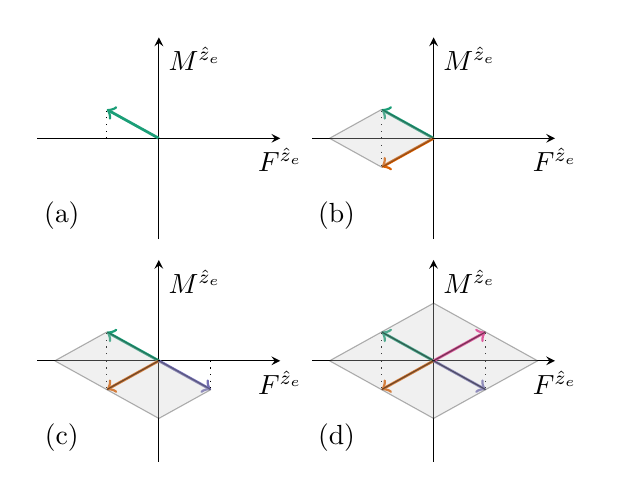
\begin{tikzpicture}
\def\scl{0.45} % define scale variable for plots

% PRACTICE PLOT
\matrix [row sep=0.25cm, column sep=0cm, style={align=center}] (my matrix) at (0,0)
{

\begin{axis}[
    view={90}{0},
    axis lines=center,
    % axis equal image,
    xlabel={$M^{\hat{x}_e}$},
    ylabel={$F^{\hat{z}_e}$},
    zlabel={$M^{\hat{z}_e}$},
    ymin=-7, ymax=7, ytick={0}, %ylabel near ticks,
    xmin=-5, xmax=10, xtick={0}, %xticklabel=$\pgfmathprintnumber{\tick}^\circ$, xlabel near ticks, 
    zmin=-7, zmax=7, ztick={0}, %z dir=reverse,
    xlabel style={anchor=north}, ylabel style={anchor=north},
    scale=\scl,
    anchor=center,
    name=plot1,
    ]
    \def\pa{(-2,-3,2)}
    \def\pb{(2,-3,-2)}
    \def\pc{(2,3,-2)}
    \def\pd{(-2,3,2)}
    \addplot3[->, line width=1pt, plgreen] coordinates {(0,0,0) \pa};
%    \addplot3[->, line width=1pt, plorange] coordinates {(0,0,0) \pb};
%    \addplot3[->, line width=1pt, plpurple] coordinates {(0,0,0) \pc};
%    \addplot3[->, line width=1pt, plpink] coordinates {(0,0,0) \pd};
    % connector lines for perspective
    \addplot3[dotted] coordinates {(0,0,0) (-2,-3,0)};
    \addplot3[dotted] coordinates {(-2,-3,0) \pa}; 
%    \addplot3[dotted] coordinates {(0,0,0) (2,-3,0)};
%    \addplot3[dotted] coordinates {(2,-3,0) \pb};
%    \addplot3[dotted] coordinates {(0,0,0) (2,3,0)};
%    \addplot3[dotted] coordinates {(2,3,0) \pc};
%    \addplot3[dotted] coordinates {(0,0,0) (-2,3,0)};
%    \addplot3[dotted] coordinates {(-2,3,0) \pd};
    % faces of shape
%    \addplot3[patch, opacity=0.3, fill=black!20, faceted color=black, patch type=rectangle] 
%        coordinates {
%                    (0,0,0) \pa (0,-6,0) \pb
%                    (0,0,0) \pb (4,0,-4) \pc
%                    (0,0,0) \pc (0,6,0) \pd
%                    (0,0,0) \pd (-4,0,4) \pa
%                    };
\end{axis};

&

\begin{axis}[
    view={90}{0},
    axis lines=center,
    % axis equal image,
    xlabel={$M^{\hat{x}_e}$},
    ylabel={$F^{\hat{z}_e}$},
    zlabel={$M^{\hat{z}_e}$},
    ymin=-7, ymax=7, ytick={0}, %ylabel near ticks,
    xmin=-5, xmax=10, xtick={0}, %xticklabel=$\pgfmathprintnumber{\tick}^\circ$, xlabel near ticks, 
    zmin=-7, zmax=7, ztick={0}, %z dir=reverse,
    xlabel style={anchor=north}, ylabel style={anchor=north},
    scale=\scl,
    anchor=center,
    name=plot2,
    ]
    \def\pa{(-2,-3,2)}
    \def\pb{(2,-3,-2)}
    \def\pc{(2,3,-2)}
    \def\pd{(-2,3,2)}
    \addplot3[->, line width=1pt, plgreen] coordinates {(0,0,0) \pa};
    \addplot3[->, line width=1pt, plorange] coordinates {(0,0,0) \pb};
%    \addplot3[->, line width=1pt, plpurple] coordinates {(0,0,0) \pc};
%    \addplot3[->, line width=1pt, plpink] coordinates {(0,0,0) \pd};
    % connector lines for perspective
    \addplot3[dotted] coordinates {(0,0,0) (-2,-3,0)};
    \addplot3[dotted] coordinates {(-2,-3,0) \pa}; 
    \addplot3[dotted] coordinates {(0,0,0) (2,-3,0)};
    \addplot3[dotted] coordinates {(2,-3,0) \pb};
%    \addplot3[dotted] coordinates {(0,0,0) (2,3,0)};
%    \addplot3[dotted] coordinates {(2,3,0) \pc};
%    \addplot3[dotted] coordinates {(0,0,0) (-2,3,0)};
%    \addplot3[dotted] coordinates {(-2,3,0) \pd};
    % faces of shape
    \addplot3[patch, opacity=0.3, fill=black!20, faceted color=black, patch type=rectangle] 
        coordinates {
                    (0,0,0) \pa (0,-6,0) \pb
%                    (0,0,0) \pb (4,0,-4) \pc
%                    (0,0,0) \pc (0,6,0) \pd
%                    (0,0,0) \pd (-4,0,4) \pa
                    };
\end{axis};


\\

\begin{axis}[
    view={90}{0},
    axis lines=center,
    % axis equal image,
    xlabel={$M^{\hat{x}_e}$},
    ylabel={$F^{\hat{z}_e}$},
    zlabel={$M^{\hat{z}_e}$},
    ymin=-7, ymax=7, ytick={0}, %ylabel near ticks,
    xmin=-5, xmax=10, xtick={0}, %xticklabel=$\pgfmathprintnumber{\tick}^\circ$, xlabel near ticks, 
    zmin=-7, zmax=7, ztick={0}, %z dir=reverse,
    xlabel style={anchor=north}, ylabel style={anchor=north},
    scale=\scl,
    anchor=center,
    name=plot3,
    ]
    \def\pa{(-2,-3,2)}
    \def\pb{(2,-3,-2)}
    \def\pc{(2,3,-2)}
    \def\pd{(-2,3,2)}
    \addplot3[->, line width=1pt, plgreen] coordinates {(0,0,0) \pa};
    \addplot3[->, line width=1pt, plorange] coordinates {(0,0,0) \pb};
    \addplot3[->, line width=1pt, plpurple] coordinates {(0,0,0) \pc};
%    \addplot3[->, line width=1pt, plpink] coordinates {(0,0,0) \pd};
    % connector lines for perspective
    \addplot3[dotted] coordinates {(0,0,0) (-2,-3,0)};
    \addplot3[dotted] coordinates {(-2,-3,0) \pa}; 
    \addplot3[dotted] coordinates {(0,0,0) (2,-3,0)};
    \addplot3[dotted] coordinates {(2,-3,0) \pb};
    \addplot3[dotted] coordinates {(0,0,0) (2,3,0)};
    \addplot3[dotted] coordinates {(2,3,0) \pc};
%    \addplot3[dotted] coordinates {(0,0,0) (-2,3,0)};
%    \addplot3[dotted] coordinates {(-2,3,0) \pd};
    % faces of shape
    \addplot3[patch, opacity=0.3, fill=black!20, faceted color=black, patch type=rectangle] 
        coordinates {
                    (0,0,0) \pa (0,-6,0) \pb
                    (0,0,0) \pb (4,0,-4) \pc
%                    (0,0,0) \pc (0,6,0) \pd
%                    (0,0,0) \pd (-4,0,4) \pa
                    };
\end{axis};

&

\begin{axis}[
    view={90}{0},
    axis lines=center,
    % axis equal image,
    xlabel={$M^{\hat{x}_e}$},
    ylabel={$F^{\hat{z}_e}$},
    zlabel={$M^{\hat{z}_e}$},
    ymin=-7, ymax=7, ytick={0}, %ylabel near ticks,
    xmin=-5, xmax=10, xtick={0}, %xticklabel=$\pgfmathprintnumber{\tick}^\circ$, xlabel near ticks, 
    zmin=-7, zmax=7, ztick={0}, %z dir=reverse,
    xlabel style={anchor=north}, ylabel style={anchor=north},
    scale=\scl,
    anchor=center,
    name=plot4,
    ]
    \def\pa{(-2,-3,2)}
    \def\pb{(2,-3,-2)}
    \def\pc{(2,3,-2)}
    \def\pd{(-2,3,2)}
    \addplot3[->, line width=1pt, plgreen] coordinates {(0,0,0) \pa};
    \addplot3[->, line width=1pt, plorange] coordinates {(0,0,0) \pb};
    \addplot3[->, line width=1pt, plpurple] coordinates {(0,0,0) \pc};
    \addplot3[->, line width=1pt, plpink] coordinates {(0,0,0) \pd};
    % connector lines for perspective
    \addplot3[dotted] coordinates {(0,0,0) (-2,-3,0)};
    \addplot3[dotted] coordinates {(-2,-3,0) \pa}; 
    \addplot3[dotted] coordinates {(0,0,0) (2,-3,0)};
    \addplot3[dotted] coordinates {(2,-3,0) \pb};
    \addplot3[dotted] coordinates {(0,0,0) (2,3,0)};
    \addplot3[dotted] coordinates {(2,3,0) \pc};
    \addplot3[dotted] coordinates {(0,0,0) (-2,3,0)};
    \addplot3[dotted] coordinates {(-2,3,0) \pd};
    % faces of shape
    \addplot3[patch, opacity=0.3, fill=black!20, faceted color=black, patch type=rectangle] 
        coordinates {
                    (0,0,0) \pa (0,-6,0) \pb
                    (0,0,0) \pb (4,0,-4) \pc
                    (0,0,0) \pc (0,6,0) \pd
                    (0,0,0) \pd (-4,0,4) \pa
                    };
\end{axis};

\\
};

\node[above] (a2) at ($ (plot1.south west) !0.1! (plot1.south east) $) {(a)};
\node[above] (b2) at ($ (plot2.south west) !0.1! (plot2.south east) $) {(b)};
\node[above] (c2) at ($ (plot3.south west) !0.1! (plot3.south east) $) {(c)};
\node[above] (d2) at ($ (plot4.south west) !0.1! (plot4.south east) $) {(d)};

\end{tikzpicture}

    \caption{An end effector is driven by the parallel combination of two pairs of FREEs with opposing chirality.
    The zonotope (grey areas) is the range of forces that can be produced by applying strictly positive pressure to the individual FREEs.
    It is spanned by the individual force vectors that each FREE produces at maximal pressure (plotted here in the color corresponding to the FREE's appearance in the diagram above).
    By constructing the zonotope for (a) one FREE, (b) two FREEs, (c) three FREEs, (d) four FREEs in parallel, one can observe that all four actuators are needed to gain full control authority over forces along and torques about the $z$-axis.
    In this poorly designed system (with fiber angles and attachments points as shown in the top diagram), the theoretical minimum of 3 actuators is not sufficient to achieve full control authority.}
    \label{fig:zntpConstructed}
\end{figure}






















\section{Experimental Evaluation}
\label{sec:experiment}
To demonstrate the viability of our modeling methodology, we show experimentally how through the deliberate combination and configuration of parallel FREEs, full control over 2DOF spacial forces can be achieved by using only the minimum combination of three FREEs.
To this end, we carefully chose the fiber angle $\Gamma$ of each of these actuators to achieve a well-balanced force zonotope (Fig.~\ref{fig:rigDiagram}).
We combined a contracting and counterclockwise twisting FREE with a fiber angle of $\Gamma = 48^\circ$, a contracting and clockwise twisting FREE with $\Gamma = -48^\circ$, and an extending FREE with $\Gamma = -85^\circ$.
All three FREEs were designed with a nominal radius of $R$ = \unit[5]{mm} and a length of $L$ = \unit[100]{mm}.
%
\begin{figure}
    \centering
    \includegraphics[width=0.75\linewidth]{figures/rigDiagram_wlabels10.pdf}
    \caption{In the experimental evaluation, we employed a parallel combination of three FREEs (top) to yield forces along and moments about the $z$-axis of an end effector.
    The FREEs were carefully selected to yield a well-balanced force zonotope (bottom) to gain full control authority over $F^{\hat{z}_e}$ and $M^{\hat{z}_e}$.
    To this end, we used one extending FREE, and two contracting FREEs which generate antagonistic moments about the end effector $z$-axis.}
    \label{fig:rigDiagram}
\end{figure}


\subsection{Experimental Setup}
To measure the forces generated by this actuator combination under a varying state $\vec{x}$ and pressure input $\vec{p}$, we developed a custom built test platform (Fig.~\ref{fig:rig}). 
%
\begin{figure}
    \centering
    \includegraphics[width=0.9\linewidth]{figures/photos/rig_labeled.pdf}
    \caption{\revcomment{1.3}{This experimental platform is used to generate a targeted displacement (extension and twist) of the end effector and to measure the forces and torques created by a parallel combination of three FREEs. A linear actuator and servomotor impose an extension and a twist, respectively, while the net force and moment generated by the FREEs is measured with a force load cell and moment load cell mounted in series.}}
    \label{fig:rig}
\end{figure}
%
In the test platform, a linear actuator (ServoCity HDA 6-50) and a rotational servomotor (Hitec HS-645mg) were used to impose a 2-dimensional displacement on the end effector. 
A force load cell (LoadStar  RAS1-25lb) and a moment load cell (LoadStar RST1-6Nm) measured the end-effector forces $F^{\hat{z_e}}$ and moments $M^{\hat{z_e}}$, respectively.
During the experiments, the pressures inside the FREEs were varied using pneumatic pressure regulators (Enfield TR-010-g10-s). 

The FREE attachment points (measured from the end effector origin) were measured to be:
\begin{align}
    \vec{d}_1 &= \bmx 0.013 & 0 & 0 \emx^T  \text{m}\\
    \vec{d}_2 &= \bmx -0.006 & 0.011 & 0 \emx^T  \text{m}\\
    \vec{d}_3 &= \bmx -0.006 & -0.011 & 0 \emx^T \text{m}
%    \vec{d}_i &= \bmx 0 & 0 & 0 \emx^T , && \text{for } i = 1,2,3
\end{align}
All three FREEs were oriented parallel to the end effector $z$-axis:
\begin{align}
    \hat{a}_i &= \bmx 0 & 0 & 1 \emx^T, \hspace{20pt} \text{for } i = 1,2,3
\end{align}
Based on this geometry, the transformation matrices $\bar{\mathcal{D}}_i$ were given by:
\begin{align}
    \bar{\mathcal{D}}_1 &= \bmx 0 & 0 & 1 & 0 & -0.013 & 0 \\ 0 & 0 & 0 & 0 & 0 & 1 \emx^T  \\
    \bar{\mathcal{D}}_2 &= \bmx 0 & 0 & 1 & 0.011 & 0.006 & 0 \\ 0 & 0 & 0 & 0 & 0 & 1 \emx^T  \\
    \bar{\mathcal{D}}_3 &= \bmx 0 & 0 & 1 & -0.011 & 0.006 & 0 \\ 0 & 0 & 0 & 0 & 0 & 1 \emx^T 
%    \bar{\mathcal{D}}_i &= \bmx 0 & 0 & 1 & 0 & 0 & 0 \\ 0 & 0 & 0 & 0 & 0 & 1 \emx^T , && \text{for } i = 1,2,3
\end{align}
These matrices were used in equation \eqref{eq:zeta} to yield the state-dependent fluid Jacobian $\bar{J}_x$ and to compute the resulting force zontopes.
%while using measured values of $\vec{\zeta}^{\,\text{meas}} (\vec{q}, \vec{P})$ and $\vec{\zeta}^{\,\text{meas}} (\vec{q}, 0)$ in \eqref{eq:fiberIso} yields the empirical measurements of the active force.



\subsection{Isolating the Active Force}
To compare our model force predictions (which focus only on the active forces induced by the fibers)
to those measured empirically on a physical system, we had to remove the elastic force components attributed to the elastomer. 
Under the assumption that the elastomer force is merely a function of the displacement $\vec{x}$ and independent of pressure $\vec{p}$ \cite{bruder2017model}, this force component can be approximated by the measured force at a pressure of $\vec{p}=0$. 
That is: 
\begin{align}
    \vec{f}_{\text{elast}} (\vec{x}) = \vec{f}_{\text{\,meas}} (\vec{x}, 0)
\end{align}
With this, the active generalized forces were measured indirectly by subtracting off the force generated at zero pressure:
\begin{align}
    \vec{f} (\vec{x}, \vec{p})  &= \vec{f}_{\text{meas}} (\vec{x}, \vec{p}) - \vec{f}_{\text{meas}} (\vec{x}, 0)     \label{eq:fiberIso}
\end{align}


%To validate our parallel force model, we compare its force predictions, $\vec{\zeta}_{\text{pred}}$, to those measured empirically on a physical system, $\vec{\zeta}_\text{meas}$. 
%From \eqref{eq:Z} and \eqref{eq:zeta}, the force at the end effector is given by:
%\begin{align}
%    \vec{\zeta}(\vec{q}, \vec{P}) &= \sum_{i=1}^n \bar{\mathcal{D}}_i \left( {\bar{J}_V}_i^T(\vec{q_i}) P_i + \vec{Z}_i^{\text{elast}} (\vec{q_i}) \right) \\
%    &= \underbrace{\sum_{i=1}^n \bar{\mathcal{D}}_i {\bar{J}_V}_i^T(\vec{q_i}) P_i}_{\vec{\zeta}^{\,\text{fiber}} (\vec{q}, \vec{P})} + \underbrace{\sum_{i=1}^n \bar{\mathcal{D}}_i \vec{Z}_i^{\text{elast}} (\vec{q_i})}_{\vec{\zeta}^{\text{elast}} (\vec{q})}   \label{eq:zetaSplit}
%     &= \vec{\zeta}^{\,\text{fiber}} (\vec{q}, \vec{P}) + \vec{\zeta}^{\text{elast}} (\vec{q})
%\end{align}
%\Dan{These will need to reflect changes made to previous section.}
%The model presented in this paper does not specify the elastomer forces, $\vec{\zeta}^{\text{elast}}$, therefore we only validate its predictions %of the fiber forces, $\vec{\zeta}^{\,\text{fiber}}$. 
%We isolate the fiber forces by noting that $\vec{\zeta}^{\text{elast}} (\vec{q}) = \vec{\zeta}(\vec{q}, 0)$ and rearranging \eqref{eq:zetaSplit}
%\begin{align}
%    \vec{\zeta}^{\,\text{fiber}} (\vec{q}, \vec{P})  &= \vec{\zeta}(\vec{q}, \vec{P}) - \vec{\zeta}(\vec{q}, 0)     \label{eq:fiberIso}
%%    \vec{\zeta}^{\,\text{fiber}}_{\text{emp}} (\vec{q}, \vec{P})  &= \vec{\zeta}_{\text{emp}}(\vec{q}, \vec{P}) - %\vec{\zeta}_{\text{emp}}(\vec{q}, 0)
%\end{align}
%Thus we measure the fiber forces indirectly by subtracting off the forces generated at zero pressure.  


\subsection{Experimental Protocol}
The force and moment generated by the parallel combination of FREEs about the end effector $z$-axis  was measured in four different geometric configurations: neutral, extended, twisted, and simultaneously extended and twisted (see Table \ref{table:RMSE} for the exact deformation amounts). 
At each of these configurations, the forces were measured at all pressure combinations in the set
\begin{align}
    \mathcal{P} &= \left\{ \bmx \alpha_1 & \alpha_2 & \alpha_3 \emx^T p^{\text{max}} \, : \, \alpha_i = \left\{ 0, \frac{1}{4}, \frac{1}{2}, \frac{3}{4}, 1 \right\} \right\}
\end{align}
with $p^{\text{max}}$ = \unit[103.4]{kPa}. 
\revcomment{3.2}{The experiment was performed twice using two different sets of FREEs to observe how fabrication variability might affect performance. The results from Trial 1 are displayed in Fig.~\ref{fig:results} and the error for both trials is given in Table \ref{table:RMSE}.}



\subsection{Results}

\begin{figure*}[ht]
\centering

\def\picScale{0.08}    % define variable for scaling all pictures evenly
\def\plotScale{0.2}    % define variable for scaling all plots evenly
\def\colWidth{0.22\linewidth}

\begin{tikzpicture} %[every node/.style={draw=black}]
% \draw[help lines] (0,0) grid (4,2);
\matrix [row sep=0cm, column sep=0cm, style={align=center}] (my matrix) at (0,0) %(2,1)
{
& \node (q1) {(a) $\Delta l = 0, \Delta \phi = 0$}; & \node (q2) {(b) $\Delta l = 5\text{mm}, \Delta \phi = 0$}; & \node (q3) {(c) $\Delta l = 0, \Delta \phi = 20^\circ$}; & \node (q4) {(d) $\Delta l = 5\text{mm}, \Delta \phi = 20^\circ$};

\\

&
\node[style={anchor=center}] {\includegraphics[width=\colWidth]{figures/photos/s0w0pic_colored.pdf}}; %\fill[blue] (0,0) circle (2pt);
&
\node[style={anchor=center}] {\includegraphics[width=\colWidth]{figures/photos/s5w0pic_colored.pdf}}; %\fill[blue] (0,0) circle (2pt);
&
\node[style={anchor=center}] {\includegraphics[width=\colWidth]{figures/photos/s0w20pic_colored.pdf}}; %\fill[blue] (0,0) circle (2pt);
&
\node[style={anchor=center}] {\includegraphics[width=\colWidth]{figures/photos/s5w20pic_colored.pdf}}; %\fill[blue] (0,0) circle (2pt);

\\

\node[rotate=90] (ylabel) {Moment, $M^{\hat{z}_e}$ (N-m)};
&
\node[style={anchor=center}] {\includegraphics[width=\colWidth]{figures/plots3/s0w0.pdf}}; %\fill[blue] (0,0) circle (2pt);
&
\node[style={anchor=center}] {\includegraphics[width=\colWidth]{figures/plots3/s5w0.pdf}}; %\fill[blue] (0,0) circle (2pt);
&
\node[style={anchor=center}] {\includegraphics[width=\colWidth]{figures/plots3/s0w20.pdf}}; %\fill[blue] (0,0) circle (2pt);
&
\node[style={anchor=center}] {\includegraphics[width=\colWidth]{figures/plots3/s5w20.pdf}}; %\fill[blue] (0,0) circle (2pt);

\\

& \node (xlabel1) {Force, $F^{\hat{z}_e}$ (N)}; & \node (xlabel2) {Force, $F^{\hat{z}_e}$ (N)}; & \node (xlabel3) {Force, $F^{\hat{z}_e}$ (N)}; & \node (xlabel4) {Force, $F^{\hat{z}_e}$ (N)};

\\
};
\end{tikzpicture}

\caption{For four different deformed configurations (top row), we compare the predicted and the measured forces for the parallel combination of three FREEs (bottom row). 
\revcomment{2.6}{Data points and predictions corresponding to the same input pressures are connected by a thin line, and the convex hull of the measured data points is outlined in black.}
The Trial 1 data is overlaid on top of the theoretical force zonotopes (grey areas) for each of the four configurations.
Identical colors indicate correspondence between a FREE and its resulting force/torque direction.}
\label{fig:results}
\end{figure*}






% & \node (a) {(a)}; & \node (b) {(b)}; & \node (c) {(c)}; & \node (d) {(d)};


For comparison, the measured forces are superimposed over the force zonotope generated by our model in Fig.~\ref{fig:results}a-~\ref{fig:results}d.
To quantify the accuracy of the model, we defined the error at the $j^{th}$ evaluation point as the difference between the modeled and measured forces
\begin{align}
%    \vec{e}_j &= \left( {\vec{\zeta}_{\,\text{mod}}} - {\vec{\zeta}_{\,\text{emp}}} \right)_j
%    e_j &= \left( F/M_{\,\text{mod}} - F/M_{\,\text{emp}} \right)_j
    e^F_j &= \left( F^{\hat{z}_e}_{\text{pred}, j} - F^{\hat{z}_e}_{\text{meas}, j} \right) \\
    e^M_j &= \left( M^{\hat{z}_e}_{\text{pred}, j} - M^{\hat{z}_e}_{\text{meas}, j} \right)
\end{align}
and evaluated the error across all $N = 125$ trials of a given end effector configuration.
% using the following metrics:
% \begin{align}
%     \text{RMSE} &= \sqrt{ \frac{\sum_{j=1}^{N} e_j^2}{N} } \\
%     \text{Max Error} &= \max \{ \left| e_j \right| : j = 1, ... , N \}
% \end{align}
As shown in Table \ref{table:RMSE}, the root-mean-square error (RMSE) is less than \unit[1.5]{N} (\unit[${8 \times 10^{-3}}$]{Nm}), and the maximum error is less than \unit[3]{N}  (\unit[${19 \times 10^{-3}}$]{Nm}) across all trials and configurations.

\begin{table}[H]
\centering
\caption{Root-mean-square error and maximum error}
\begin{tabular}{| c | c || c | c | c | c|}
    \hline
     & \rule{0pt}{2ex} \textbf{Disp.} & \multicolumn{2}{c |}{\textbf{RMSE}} & \multicolumn{2}{c |}{\textbf{Max Error}} \\ 
     \cline{2-6}
     & \rule{0pt}{2ex} (mm, $^\circ$) & F (N) & M (Nm) & F (N) & M (Nm) \\
     \hline
     \multirow{4}{*}{\rotatebox[origin=c]{90}{\textbf{Trial 1}}}
     & 0, 0 & 1.13 & $3.8 \times 10^{-3}$ & 2.96 & $7.8 \times 10^{-3}$ \\
     & 5, 0 & 0.74 & $3.2 \times 10^{-3}$ & 2.31 & $7.4 \times 10^{-3}$ \\
     & 0, 20 & 1.47 & $6.3 \times 10^{-3}$ & 2.52 & $15.6 \times 10^{-3}$\\
     & 5, 20 & 1.18 & $4.6 \times 10^{-3}$ & 2.85 & $12.4 \times 10^{-3}$ \\  
     \hline
     \multirow{4}{*}{\rotatebox[origin=c]{90}{\textbf{Trial 2}}}
     & 0, 0 & 0.93 & $6.0 \times 10^{-3}$ & 1.90 & $13.3 \times 10^{-3}$ \\
     & 5, 0 & 1.00 & $7.7 \times 10^{-3}$ & 2.97 & $19.0 \times 10^{-3}$ \\
     & 0, 20 & 0.77 & $6.9 \times 10^{-3}$ & 2.89 & $15.7 \times 10^{-3}$\\
     & 5, 20 & 0.95 & $5.3 \times 10^{-3}$ & 2.22 & $13.3 \times 10^{-3}$ \\  
     \hline
\end{tabular}
\label{table:RMSE}
\end{table}

\begin{figure}
    \centering
    \includegraphics[width=\linewidth]{figures/photos/buckling.pdf}
    \caption{At high fluid pressure the FREE with fiber angle of $-85^\circ$ started to buckle.  This effect was less pronounced when the system was extended along the $z$-axis.}
    \label{fig:buckling}
\end{figure}

%Experimental precision was limited by unmodeled material defects in the FREEs, as well as sensor inaccuracy. While the commercial force and moment sensors used have a quoted accuracy of 0.02\% for the force sensor and 0.2\% for the moment sensor (LoadStar Sensors, 2015), a drifting of up to 0.5 N away from zero was noticed on the force sensor during testing.

It should be noted, that throughout the experiments, the FREE with a fiber angle of $-85^\circ$ exhibited noticeable buckling behavior at pressures above $\approx$ \unit[50]{kPa} (Fig.~\ref{fig:buckling}). 
This behavior was more pronounced during testing in the non-extended configurations (Fig.~\ref{fig:results}a~and~\ref{fig:results}c). 
The buckling might explain the noticeable leftward offset of many of the points in Fig.~\ref{fig:results}a and Fig.~\ref{fig:results}c, since it is reasonable to assume that buckling reduces the efficacy of of the FREE to exert force in the direction normal to the force sensor. 

\begin{figure}
    \centering
    \includegraphics[width=\linewidth]{figures/zntp_vs_x4.pdf}
    \caption{A visualization of how the \emph{force zonotope} of the parallel combination of three FREEs (see Fig.~\ref{fig:rig}) changes as a function of the end effector state $x$. One can observe that the change in the zonotope ultimately limits the work-space of such a system.  In particular the zonotope will collapse for compressions of more than \unit[-10]{mm}.  For \revcomment{2.5}{scale and comparison, the convex hulls of the measured points from Fig.~\ref{fig:results}} are superimposed over their corresponding zonotope at the configurations that were evaluated experimentally.}
    % \marginnote{\#2.5}
    \label{fig:zntp_vs_x}
\end{figure}
% \vspace{-0.5em}
\section{Conclusion}
% \vspace{-0.5em}
Recent advances in multimodal single-cell technology have enabled the simultaneous profiling of the transcriptome alongside other cellular modalities, leading to an increase in the availability of multimodal single-cell data. In this paper, we present \method{}, a multimodal transformer model for single-cell surface protein abundance from gene expression measurements. We combined the data with prior biological interaction knowledge from the STRING database into a richly connected heterogeneous graph and leveraged the transformer architectures to learn an accurate mapping between gene expression and surface protein abundance. Remarkably, \method{} achieves superior and more stable performance than other baselines on both 2021 and 2022 NeurIPS single-cell datasets.

\noindent\textbf{Future Work.}
% Our work is an extension of the model we implemented in the NeurIPS 2022 competition. 
Our framework of multimodal transformers with the cross-modality heterogeneous graph goes far beyond the specific downstream task of modality prediction, and there are lots of potentials to be further explored. Our graph contains three types of nodes. While the cell embeddings are used for predictions, the remaining protein embeddings and gene embeddings may be further interpreted for other tasks. The similarities between proteins may show data-specific protein-protein relationships, while the attention matrix of the gene transformer may help to identify marker genes of each cell type. Additionally, we may achieve gene interaction prediction using the attention mechanism.
% under adequate regulations. 
% We expect \method{} to be capable of much more than just modality prediction. Note that currently, we fuse information from different transformers with message-passing GNNs. 
To extend more on transformers, a potential next step is implementing cross-attention cross-modalities. Ideally, all three types of nodes, namely genes, proteins, and cells, would be jointly modeled using a large transformer that includes specific regulations for each modality. 

% insight of protein and gene embedding (diff task)

% all in one transformer

% \noindent\textbf{Limitations and future work}
% Despite the noticeable performance improvement by utilizing transformers with the cross-modality heterogeneous graph, there are still bottlenecks in the current settings. To begin with, we noticed that the performance variations of all methods are consistently higher in the ``CITE'' dataset compared to the ``GEX2ADT'' dataset. We hypothesized that the increased variability in ``CITE'' was due to both less number of training samples (43k vs. 66k cells) and a significantly more number of testing samples used (28k vs. 1k cells). One straightforward solution to alleviate the high variation issue is to include more training samples, which is not always possible given the training data availability. Nevertheless, publicly available single-cell datasets have been accumulated over the past decades and are still being collected on an ever-increasing scale. Taking advantage of these large-scale atlases is the key to a more stable and well-performing model, as some of the intra-cell variations could be common across different datasets. For example, reference-based methods are commonly used to identify the cell identity of a single cell, or cell-type compositions of a mixture of cells. (other examples for pretrained, e.g., scbert)


%\noindent\textbf{Future work.}
% Our work is an extension of the model we implemented in the NeurIPS 2022 competition. Now our framework of multimodal transformers with the cross-modality heterogeneous graph goes far beyond the specific downstream task of modality prediction, and there are lots of potentials to be further explored. Our graph contains three types of nodes. while the cell embeddings are used for predictions, the remaining protein embeddings and gene embeddings may be further interpreted for other tasks. The similarities between proteins may show data-specific protein-protein relationships, while the attention matrix of the gene transformer may help to identify marker genes of each cell type. Additionally, we may achieve gene interaction prediction using the attention mechanism under adequate regulations. We expect \method{} to be capable of much more than just modality prediction. Note that currently, we fuse information from different transformers with message-passing GNNs. To extend more on transformers, a potential next step is implementing cross-attention cross-modalities. Ideally, all three types of nodes, namely genes, proteins, and cells, would be jointly modeled using a large transformer that includes specific regulations for each modality. The self-attention within each modality would reconstruct the prior interaction network, while the cross-attention between modalities would be supervised by the data observations. Then, The attention matrix will provide insights into all the internal interactions and cross-relationships. With the linearized transformer, this idea would be both practical and versatile.

% \begin{acks}
% This research is supported by the National Science Foundation (NSF) and Johnson \& Johnson.
% \end{acks}

% \addtolength{\textheight}{-12cm}   % This command serves to balance the column lengths
%                                   % on the last page of the document manually. It shortens
%                                   % the textheight of the last page by a suitable amount.
%                                   % This command does not take effect until the next page
%                                   % so it should come on the page before the last. Make
%                                   % sure that you do not shorten the textheight too much.

% \section{Acknowledgement}
\label{sec:conclusion}
This work is supported by National Natural Science Foundation of China (62076144), Shenzhen Key Laboratory of next generation interactive media innovative technology (ZDSYS20210623092001004),\\ Shenzhen Science and Technology Program (WDZC2022081614051\\5001) and Tencent AI Lab Rhino-Bird Focused Research Program (RBFR2022005).


\bibliographystyle{IEEEtran}
\bibliography{references}


\end{document}


